\chapter{Convergence of MOC Source Iteration}
\label{chap:moc-convergence}

In the previous chapters, the implementation of methods in OpenMOC has been discussed in great detail. All of these methods rely on the \ac{MOC} form of the transport equation presented in Chapter~\ref{chap:moc}. More specifically, these methods rely on the source iteration form the \ac{MOC} equations, possibly used in conjunction with \ac{CMFD} acceleration discussed in Chapter~\ref{chap:cmfd}. In this chapter, the convergence of source iteration with and without \ac{CMFD} acceleration is addressed. While convergence is straightforward for physical cross-sections, the transport correction discussed in Section~\ref{sec:transport-correction} can cause convergence issues. 

In Section~\ref{sec:source-iteration-intro}, the multi-group transport problem is formalized in matrix form which forms the basis of discussing convergence of source iteration. Section~\ref{sec:equiv-cpm} relates multi-group transport forms to collision probabilities, allowing for an analytical description of iteration matrix elements. Section~\ref{sec:moc-iteration-schemes} discusses methods to solve the resulting system of equations, focusing on source iteration. Theoretical issues with source iteration are discussed for transport-corrected cross-sections. Then, in Section~\ref{sec:diagonal-stabilization} a solution is proposed, termed diagonal stabilization. Finally, Section~\ref{sec:convergence-results} demonstrates convergence issues of source iteration on realistic problems and the ability of diagonal stabilization to fix the convergence issues.

\section{Introduction}
\label{sec:source-iteration-intro}

The multi-group transport equation can be solved by a variety of methods, including \ac{MOC}. Many of these methods discretize the transport equation in some fashion and solve a linear system of the form
\begin{equation}
	\boldsymbol{\phi} = J \left(\frac{1}{k} F + S \right) \boldsymbol{\phi}
	\label{eq:si-transport}
\end{equation}
where $\boldsymbol{\phi}$ represents the vector of all scalar fluxes, $J$ is the transport sweep matrix, $F$ is the fission matrix, $S$ is the scattering matrix, and $k$ is the eigenvalue. 

In many efficient transport solvers, these matrices are not explicitly formed but rather they implicitly solve these equations with sweeps taking the place of explicit formulation of the matrix elements. Therefore, these matrices are often presented as operators rather than matrices, but the underlying matrix elements could be computed if desired. 

For physical cross-sections, the matrices $J$, $F$, and $S$ are all positive.
\begin{equation}
\begin{split}
\Sigma_{\textit{tr}, i, g} = \Sigma_{t, i, g} -  \Delta \Sigma_{\textit{tr}, i, g} \\
\tilde{\Sigma}_{s, i}^{g \rightarrow g} = \Sigma_{s, i}^{g \rightarrow g} -  \Delta \Sigma_{\textit{tr}, i, g}
\end{split}
\label{eq:total-xs}
\end{equation}

When using large numbers of energy groups, the within-group scattering cross-sections can become small, and the modified within-group scattering cross-section can become negative with transport correction. Tabuchi discovered negative within-group scattering cross-sections to be an issue when converging inner within-group scattering iterations of \ac{MOC}~\cite{ty-problem}. Specifically, it was identified that the inner iteration matrix could have a spectral radius greater than unity, causing the system not to converge. Tabuchi later proposed a stabilization technique for inner iterations~\cite{ty-solution}.

In this chapter, the ideas presented by Tabuchi are expanded to explain the observed convergence behavior of source iteration without inner iterations. Convergence is analyzed with transport corrected cross-sections. Realistic full core cases are presented that observe the failed convergence behavior and a new stabilizing method is proposed that stabilizes source iteration.

\section{Equivalence of Collision Probability Methods}
\label{sec:equiv-cpm}

Deterministic methods such as flat source \ac{MOC} or step characteristics are equivalent to the collision probability form, aside from discretization errors~\cite{ty-problem}. Although collision probabilities do not explicitly enter the transport method, the neutron balance equation takes the form in Eq.~\ref{eq:cpm-form}:
\begin{equation}
	\Sigma_{\textit{tr}, i, g} \phi_{i,g} V_i = \sum_j P_{ji, g} q_{j,g} V_j
	\label{eq:cpm-form}
\end{equation}
where $P_{ji,g}$ represents the collision probability of a neutron of energy group $g$ from region $j$ to region $i$, $V_i$ represents the volume of region $i$, $q_{i,g}$ represents the neutron source and $\phi_{i,g}$ represents the average scalar flux in region $i$ and group $g$. In general, the neutron source can be computed by summing contributions from all $G$ energy groups as
\begin{equation}
	q_{i,g} = \sum_{g'=1}^G \left( \Sigma_{s,i}^{g'\rightarrow g} \phi_{i,g'} + \chi_{i,g} \nu \Sigma_{f,i,g'} \phi_{i,g'} \right)
\end{equation}
where $\Sigma_{s,i}^{g'\rightarrow g}$ is the scattering cross-section in region $i$ from group $g'$ to group $g$, $\chi_{i,g}$ is the fission emission probability for group $g$ in region $i$, and $\nu \Sigma_{f,i,g'}$ is the fission production in region $i$ from group $g'$. Combining this definition with Eq.~\ref{eq:cpm-form}, as well as the reciprocity relationship, 
\begin{equation}
	P_{ij, g} \Sigma_{\textit{tr}, i, g} V_i = P_{ji, g} \Sigma_{\textit{tr}, j, g} V_j,
	\label{eq:reciprocity}
\end{equation}
neutron balance can be presented in the form of Eq.~\ref{eq:cpm-balance}.
\begin{equation}
	\phi_{i,g} = \sum_j \frac{P_{ij, g} \sum_{g'=1}^G \left( \Sigma_{s,j}^{g'\rightarrow g} \phi_{j,g'} + \chi_{j,g} \nu \Sigma_{f,j,g'} \phi_{j,g'} \right)}{\Sigma_{\textit{tr}, j, g}} 
	\label{eq:cpm-balance}
\end{equation}
Notice that this is in the form of Eq.~\ref{eq:si-transport}. Therefore, the matrix $A = J\left(\frac{1}{k}F + S\right)$, with rows and columns indexed by $(i, g)$  where $i$ is the region and $g$ is the energy group, can be expressed as
\begin{equation}
	A_{(i,g), (j, g')} = P_{ij}^g \left(\frac{\chi_{j,g} \nu\Sigma_{f,j,g'} / k + \Sigma_{s,j}^{g' \rightarrow g}}{\Sigma_{\textit{tr}, j, g}}\right).
	\label{eq:a-matrix}
\end{equation}
Matrix $A$ is square and dense with length equal to the number of scalar fluxes. 

\section{Iteration Schemes}
\label{sec:moc-iteration-schemes}

\subsection{Power Method}

Often an iterative process is performed in which a new source distribution is computed at each iteration, yielding a new estimate of the associated scalar flux distribution. Therefore, solving the transport equation in this form where source terms are lagged is termed \textit{source iteration}.

One method to solve a system of the form given in Eq.~\ref{eq:si-transport} is the power method, which yields the dominant eigenvector corresponding to the steady-state flux distribution. To invoke the power method, Eq.~\ref{eq:si-transport} can be re-arranged to the form in Eq.~\ref{eq:eigenvalue} where $I$ represents the identity matrix~\cite{kords-book}.
\begin{equation}
\begin{split}
Z \equiv \left(I-JS\right)^{-1} JF \\
Z \boldsymbol{\phi} =  k \boldsymbol{\phi}
\end{split}
\label{eq:eigenvalue}
\end{equation}
With the power method scheme, repeated multiplication by $Z$ yields the dominant eigenvector~\cite{numerical-analysis}. Rather than performing strict power method iterations, the estimate of the eigenvalue $k_n$ at iteration $n$ is often included in the source. This scheme is presented in Eq.~\ref{eq:power-method}. These iterations are often termed \textit{outer iterations}.
\begin{equation}
\boldsymbol{\phi}_{n+1} =  \left(I-JS\right)^{-1} J\frac{F}{k_n} \boldsymbol{\phi}_n
\label{eq:power-method}
\end{equation}
Since explicitly taking the matrix inverse of $I-JS$ is unwise, an iterative scheme is necessary to solve the linear system. In many transport methods, such as \ac{MOC}, computing the elements of $J$ can be as expensive as computing a matrix vector product~\cite{transport-sweeps}. In addition, each matrix-vector product with matrix $J$ is usually quite expensive (often termed \textit{transport sweeps}). Therefore, few methods are available to efficiently solve the linear system in practice. 

\subsection{Source Iteration}

Note that in this notation the neutron source $\mathbf{q}$ can be computed as 
\begin{equation*}
	\mathbf{q} = \left(\frac{1}{k} F + S \right) \boldsymbol{\phi}. 
\end{equation*}
The transport sweep matrix $J$ therefore yields the scalar flux distribution associated with the computed source distribution. 

An alternative way to solve the transport equation is to directly apply the transport sweep to the full neutron source. The eigenvalue problem in Eq.~\ref{eq:si-transport} is iteratively solved with the left hand side updated and the right hand side lagged as
\begin{equation}
	\boldsymbol{\phi}_{n+1} =  J\left(\frac{F\boldsymbol{\phi}_n}{k_n} + S\boldsymbol{\phi}_n\right).
	\label{eq:power-method-full-source}
\end{equation}
It is important to note that this process is non-linear due to the iteration matrix $J\left(\frac{1}{k_n} F + S\right)$ being dependent on the iteration number $n$. To simplify this relationship, assume that the eigenvalue $k$ is perfectly known to be $k_{\textit{crit}}$, the eigenvalue associated with the dominant mode of the system. In reality, the exact value of $k_{\textit{crit}}$ is not known a priori but observations and intuition suggests that it does not strongly impact convergence. With the eigenvalue fixed, the system becomes 
\begin{equation}
	\boldsymbol{\phi}_{n+1} =  A \boldsymbol{\phi}_n
\end{equation}
where matrix $A$ is defined in Eq.~\ref{eq:a-matrix} with $k = k_{\textit{crit}}$. This process is equivalent to power method iterations with the matrix $A$, which converges to the eigenvector associated with the dominant eigenvalue of $A$. Since $k_{\textit{crit}}$ is the dominant eigenvalue of the original system, 1.0 must be an eigenvalue of $A$. In addition, if an everywhere positive solution exists, it must be associated with the physical solution.

Recall from Eq.~\ref{eq:a-matrix} that the iteration matrix $A$ is everywhere positive and real as long as the within-group scattering cross-section is positive. According to the Perron-Frobenius Theorem~\cite{perron-frobenius}, square matrices of all positive real entries have a unique largest real eigenvalue which is dominant and associated with an everywhere positive eigenvector. In addition, all other eigenvectors must have a negative component. Without transport correction, the iteration matrix $A$ is an all positive and real matrix, implying that the largest eigenvalue is 1.0 and is associated with the physical solution. Therefore, the process detailed in Eq.~\ref{eq:power-method-full-source} will converge to the physical solution.

However, with the transport correction, it is possible to have negative within-group scattering causing this criteria not to hold. If this criteria does not hold, the system might still converge, but convergence cannot be guaranteed under the Perron-Frobenius Theorem. Therefore, the iteration scheme should be updated to ensure convergence. 

\section{Stabilization of Source Iteration}
\label{sec:diagonal-stabilization}

Note that Eq.~\ref{eq:damped-transport} is a mathematically valid rewriting of Eq.~\ref{eq:si-transport} for \textit{any matrix} $D$ where $I+D$ is invertible. 
\begin{equation}
	\boldsymbol{\phi} = (I+D)^{-1} J \left(\frac{1}{k} F + S + D\right) \boldsymbol{\phi}
	\label{eq:damped-transport}
\end{equation}
Next, the same source iteration scheme is applied where the left hand side is updated with the right hand side constant. Since $I+D$ needs to be easily invertible for this new scheme to be efficient, $D$ is chosen to be diagonal. The convergence discussion then follows the same discussion as before except the new iteration matrix  now has the form $\tilde{A} = (I+D)^{-1} J \left(\frac{1}{k_{\textit{crit}}} F + S + D\right)$  with the matrix $\tilde{A}$ is described by
\begin{equation}
	\tilde{A}_{(i,g), (j, g')} = \frac{1}{1 + D_{(i,g), (i,g)}}\left[P_{ij}^g \left(\frac{\chi_{j,g} \nu\Sigma_{f,j,g'} / k_{\textit{crit}} + \Sigma_{s,j}^{g' \rightarrow g}}{\Sigma_{\textit{tr}, j, g}}\right) + D_{(i,g), (j, g')}\right]
	\label{eq:a-tilde}
\end{equation}
where the rows and columns are again indexed by region, energy group pairs. The diagonal elements of $D$ are chosen to be:
\begin{equation}
	D_{(i,g), (i,g)} = \left\{\begin{array}{lr}
		\frac{-\rho \Sigma_{s,i}^{g \rightarrow g}}{\Sigma_{\textit{tr}, i, g}} , & \text{for } \Sigma_{s,i}^{g \rightarrow g} < 0\\
		0, & \text{otherwise}
	\end{array}\right.
	\label{eq:d-matrix}
\end{equation}
where the damping coefficient $\rho$ is a positive value chosen by the user. For $\rho = 1$, the diagonal update ensures that there are no negative diagonal elements in the iteration matrix. The diagonal stabilization scheme has the effect of shifting the iteration matrix eigenvalues to be more positive. The intuition for this shift is due to the Gershgorin Disk Theorem where eigenvalues exist in disks around diagonal elements. Since the diagonal elements are positively increased and all matrix elements are contracted, the Gershgorin Disks are likewise shifted positively with their radii contracted. While this improves stability, it also tightens the positive-eigenvalue modes, causing larger dominance ratios in the iteration matrix, and slower convergence. Therefore, $\rho$ should be chosen to be small while still ensuring convergence. 

\section{Convergence Results}
\label{sec:convergence-results}

In order to test the convergence behavior of the stabilization methods, the stabilization methods were implemented in OpenMOC~\cite{openmoc}, a \ac{MOC} neutron transport solver. In particular, this analysis will focus on the 3D \ac{MOC} solver~\cite{openmoc-3dmoc} which has recently proven the ability to solve full core \ac{PWR} problems~\cite{openmoc-beavrs}. The cross-sections used in this analysis are generated using the OpenMC MGXS framework~\cite{will} which uses tallied Monte Carlo reaction rates to form cross-sections.

The transport correction for most materials in this analysis is taken from the P0-corrected OpenMC MGXS tallies. However, the water transport correction, which is the most vital to obtaining accurate results, uses the CASMO methodology~\cite{casmo-xs} which has recently been outlined for pure hydrogen~\cite{johnny}.

This section focuses on results for realistic reactor physics problems. All results use the 3D \ac{MOC} solver of OpenMOC with 32 azimuthal angles, 0.1 cm radial ray spacing, 6 polar angles (Gauss-Legendre quadrature), and 1.5 cm axial ray spacing. While finer \ac{MOC} parameters would be necessary to accurately the solution, the convergence has not been observed to change substantially from refining \ac{MOC} parameters beyond these values. The source region mesh for all problems has 4 sectors in fuel and 8 sectors in the moderator for pin-cells. All source regions are 2.0 cm tall. 

\subsection{Single Assembly with Axial Water Reflectors}
\label{sec:sa-axial-ref}

While OpenMOC is capable of solving full core \ac{PWR} problems, this analysis will start by focusing on a 3D single assembly model, which is computationally less expensive, in order to observe longer iteration histories. The single assembly model is 400 cm in axial height with an active fuel height of 366 cm and an assembly pitch of 21.42 cm. It is simulated with vacuum boundaries in the axial directions and reflective boundaries in the radial directions. The assembly incorporates the full geometric detail, including grid spacers. Outside the core, full geometrical detail is also captured including support plate nozzles and, most notably, water reflectors of approximately 20 cm above and below the fuel.

To analyze the convergence behavior, an error metric is needed. Usually, error is analyzed in terms of RMS error in the fission distribution over all fissile regions.  This requires a having a reference solution to be the fission distribution of tightly converged case. 


\subsubsection{Source Iteration Convergence without CMFD Acceleration}

The single assembly model is first analyzed using pure source iteration, without any \ac{CMFD} acceleration. In order to focus on the asymptotic convergence behavior, rather than the behavior far from convergence, the \ac{MOC} simulations start with a \textit{good guess} of the scalar flux distribution. Specifically, a converging simulation where the error drops below $3\times 10^{-5}$ on RMS fission rate error is chosen as the starting point.

The convergence behavior is presented in Figure~\ref{fig:no-cmfd} in which the relative error is plotted as a function of iteration number for a variety of stabilizing schemes.
\begin{figure}[ht!]
	\centering
	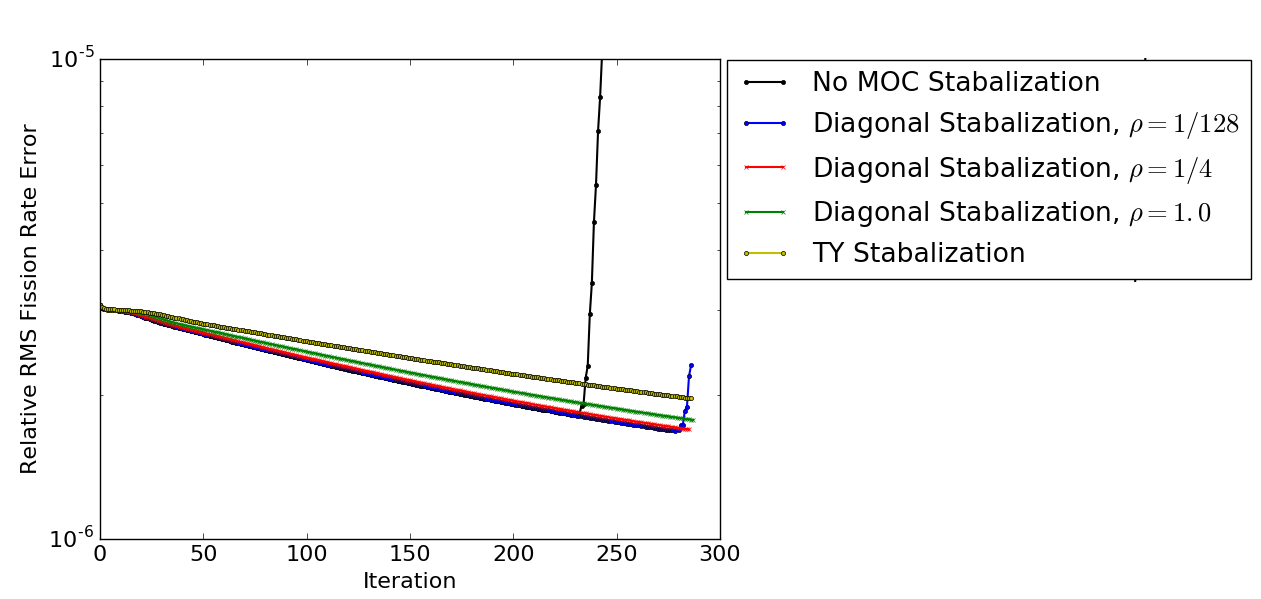
\includegraphics[width=1.0\linewidth]{figures/convergence/no_cmfd.png}
	\caption{Convergence behavior of different stabilization schemes. TY Stabalization refers to the approach presented by Tabuchi, et. al~\cite{ty-solution} whereas Diagonal Stabilization refers to the approach presented in this paper with damping coefficient $\rho$.}
	\label{fig:no-cmfd}
\end{figure}
Notice that the case without stabilization diverges while all the stabilization cases converge except for the new diagonal stabilization scheme with damping factor $\rho = 1/128$. This is expected since as $\rho$ approaches zero as the stabilization method becomes equivalent to source iteration without stabilization. This clearly shows that this problem requires stabilization to converge with source iteration. In addition, the more conservative the stabilization scheme, the more convergence is slowed. The scheme proposed by Tabuchi slows convergence the most. The diagonal damping scheme hinders convergence significantly less, especially for $\rho < 1$. 

\subsubsection{Convergence with CMFD Acceleration}

Often \ac{CMFD} acceleration is necessary to achieve reasonable convergence on practical reactor physics problems. \ac{CMFD} acceleration is implemented in OpenMOC with damping on the current correction term~\cite{smith_cmfd}, often termed the \ac{CMFD} relaxation factor. When \ac{CMFD} acceleration is applied, the behavior is much more difficult to analyze since \ac{CMFD} is a non-linear process. Therefore, discussion of \ac{CMFD} results will focus on hypotheses to explain the observed results rather than rigorous analysis. In this study, the \ac{CMFD} mesh is always chosen to be a uniform mesh with cells of pin-cell pitch in the radial dimensions and 2.0 cm in the axial dimension. In addition, a relaxation factor of 0.7 is applied to the \ac{CMFD} acceleration scheme for computing corrected diffusion coefficients. 

Many \ac{CMFD} implementations choose to collapse to a fewer number of energy groups in order to improve the speed of the CMFD solver. While the CMFD equations are computationally less expensive in collapsed few-group structures, it is possible that collapsing group structures could cause slower convergence by not fully resolving spectral effects. In this study, a variety of \ac{CMFD} group structures are presented. While the \ac{MOC} calculation always uses a 70 group structure, \ac{CMFD} group structures are formed with $G_C$ \ac{CMFD} groups, with group ranges taken from the CASMO 4 Manual~\cite{casmo-xs}.

The results with \ac{CMFD} applied and \textit{without} any \ac{MOC} source iteration stabilization are shown in Figure~\ref{fig:sa-cmfd-no-stab} for a variety of \ac{CMFD} group structures with the error once again relative to a tightly converged reference.
\begin{figure}[ht!]
	\centering
	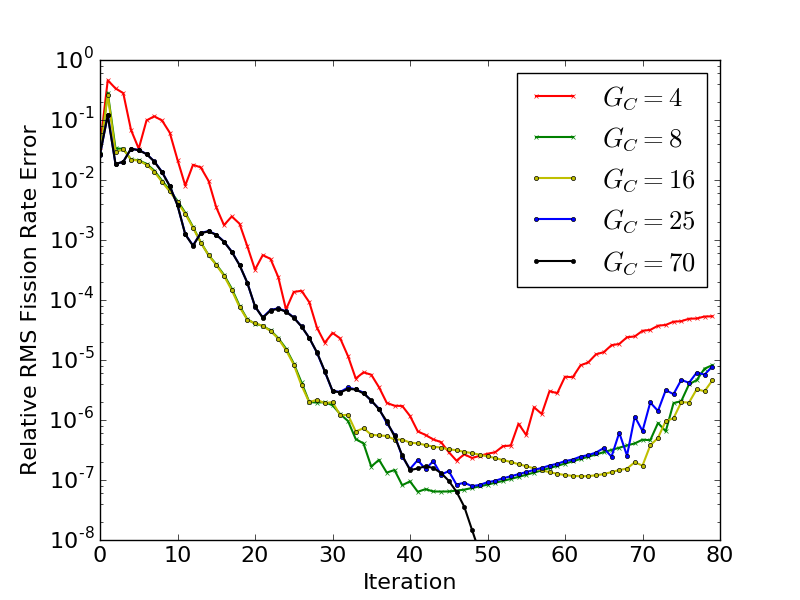
\includegraphics[width=0.65\linewidth]{figures/convergence/sa_no_stab_cmfd.png}
	\caption{Convergence behavior for a variety of \ac{CMFD} group structures with $G_C$ \ac{CMFD} groups and \textit{without} \ac{MOC} source iteration stabilization.}
	\label{fig:sa-cmfd-no-stab}
\end{figure}
As expected, most of the convergence histories have trouble converging. This is likely due to the convergence issue observed with pure source iteration. However, the 70 group \ac{CMFD} scheme appears to be stable. It is important to remember that the \ac{CMFD} equations do not suffer from the issue of a negative dominant eigenvalue in the source iteration scheme since since they solve an alternate form of the original eigenvalue system with standard eigenvalue solver techniques. 

If 70 group \ac{CMFD} is driving the convergence process, then the instability in the underlying source iteration technique might be overcome by the \ac{CMFD} acceleration prolongation update in which \ac{MOC} scalar fluxes are updated with the \ac{CMFD} solution. One way of interpreting this behavior is to think of the convergence as being dominated by the \ac{CMFD} acceleration where \ac{MOC} transport sweeps are used purely to resolve local behavior, integrate reaction rates to form \ac{CMFD} cross-sections, and tally currents crossing \ac{CMFD} mesh surfaces. 

However, with a reduced \ac{CMFD} group structure, the flux distribution in energy within a single \ac{CMFD} group \textit{must} be resolved by the \ac{MOC} source iteration process unless an effective energy interpolation can be formed during the \ac{CMFD} prolongation stage. Since the underlying \ac{MOC} source iteration process is unstable, any reliance on the process for convergence using a reduced group structure should lead to instability.

\subsubsection{Convergence with CMFD Acceleration and Source Iteration Stabilization}

To verify that the convergence issue can be remedied with \ac{MOC} source iteration stabilization, the same test is conducted but using diagonal stabilization with $\rho = 1/4$. For pure source iteration, this scheme was able to stabilize source iteration, as previously shown in Figure~\ref{fig:no-cmfd}. The results using this stabilization with \ac{CMFD} acceleration are shown in Figure~\ref{fig:sa-cmfd-stab}. As expected, the \ac{MOC} source iteration stabilization fixes the convergence issues for all \ac{CMFD} group structures, indicating that the convergence issue was caused by the underlying \ac{MOC} source iteration.
\begin{figure}[ht!]
	\centering
	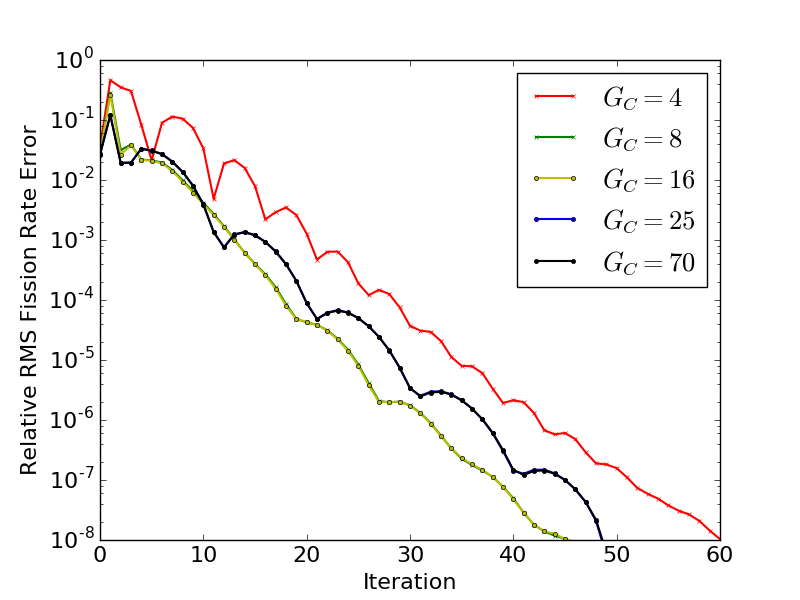
\includegraphics[width=0.65\linewidth]{figures/convergence/sa_stab_cmfd.png}
	\caption{Convergence behavior for a variety of \ac{CMFD} group structures with $G_C$ \ac{CMFD} groups and \textit{with} Diagonal \ac{MOC} source iteration stabilization ($\rho = 1/4$).}
	\label{fig:sa-cmfd-stab}
\end{figure}

\subsection{Single Assembly without Axial Water Reflectors}
\label{sec:sa-no-axial-ref}

Next, the same single assembly model is studied but without the axial water reflectors. Vacuum boundary conditions are placed at the top and bottom of the active fuel. All other geometric and material data is unchanged. This model is run \textit{without} source iteration stabilization. The results with \ac{CMFD} acceleration for a variety of \ac{CMFD} group structures are presented in Figure~\ref{fig:truncated-convergence}.
\begin{figure}[ht!]
	\centering
	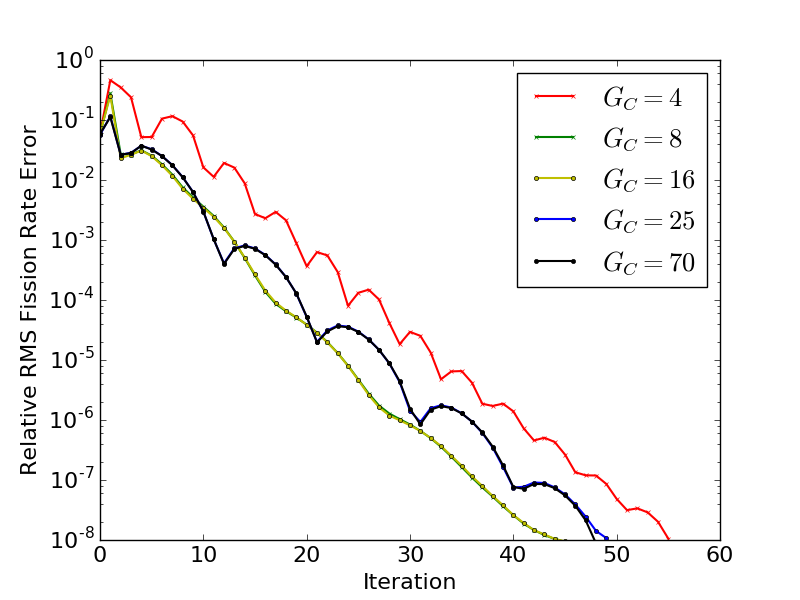
\includegraphics[width=0.65\linewidth]{figures/convergence/sa_trunc_no_stab.png}
	\caption{Convergence behavior for the single assembly \textit{without} axial reflectors with a variety of \ac{CMFD} group structures with $G_C$ \ac{CMFD} groups and \textit{without} \ac{MOC} source iteration stabilization.}
	\label{fig:truncated-convergence}
\end{figure}
Notice that the convergence issues are not present in this model. This indicates the issue is caused by the axial water reflectors. More generally, it appears to be a problem with deep water reflectors that have negative cross-sections. Recall from the theory discussion that iteration matrix components in Eq.~\ref{eq:a-matrix} were formed with the product of collision probability and self-scattering cross-sections. In deep water reflectors, the probability of transport between water regions containing negative cross-sections is significantly higher than in the active fuel where many neutrons collide with fuel. This motivates the idea of neutron behavior in deep reflectors causing the instability. 

\subsection{Full Core Behavior}

The previous results were focused on a single assembly with and without axial reflectors which proved the existence of source iteration instability. Since this issue seems to only appear at very low errors, the reader might judge this issue to be purely academic. However, for problems where deeper reflectors exist, such as a typical full core \ac{PWR} problem, this issue is exacerbated. In this last results section, the full core \ac{BEAVRS} benchmark is simulated using the same cross-section set applied in the single assembly studies. 

The model is again 400 cm in axial height with an active fuel height of 366 cm. The model extent in the radial plane is the size of $17\times 17$ assembly widths with each assembly again having a width of 21.54 cm. Since the \ac{BEAVRS} model only has 15 assemblies on the major axis, the model guarantees at least one assembly width of water reflector outside the core in every direction. Since the simulated geometry is square in the radial plane, the corners have very deep water reflectors. In general, vacuum boundaries are assumed on all surfaces. The geometry outside the core is radially discretized into square regions of length equal to $1/3$ of the pin-cell pitch (which is 1.26 cm).

\subsubsection{2D Extruded Model}

Before simulating the explicit 3D model, a 2D extruded model is constructed to observe the convergence behavior. This model takes a radial slice of the core that does not contain grid spacers and extruded the slice 10 cm in the axial direction, applying reflective boundaries on the top and bottom. This essentially converts the 3D problem into a 2D problem. Still, the problem is solved using the 3D \ac{MOC} solver. The results are shown in Figure~\ref{fig:fc-2D}. 
\begin{figure}[ht!]
	\centering
	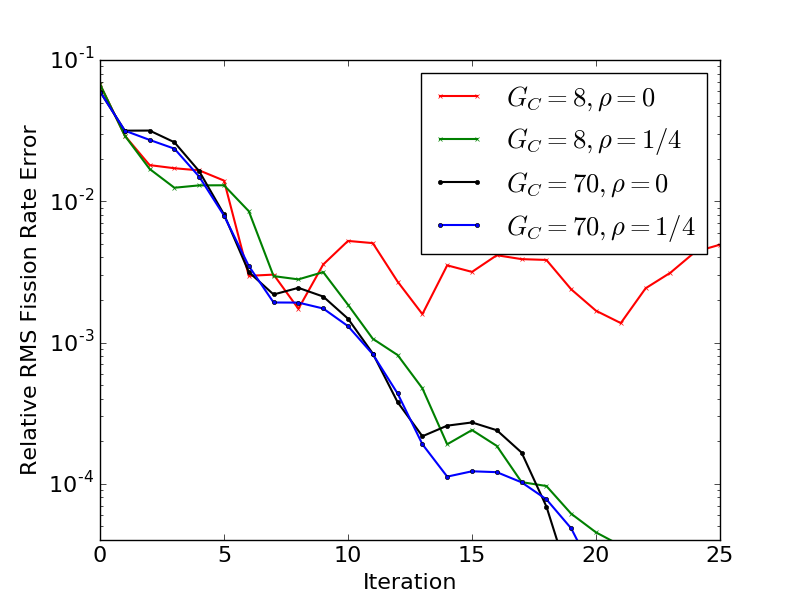
\includegraphics[width=0.65\linewidth]{figures/convergence/fc_2D.png}
	\caption{Convergence behavior of \ac{CMFD} group structures with $G_C$ \ac{CMFD} groups and Diagonal \ac{MOC} source iteration stabilization with stabilization coefficient $\rho$.}
	\label{fig:fc-2D}
\end{figure}
The simulation is run with 8 group and 70 group \ac{CMFD} with Diagonal Stabilization. The damping coefficient $\rho$ is chosen for both cases to be zero (equivalent to no stabilization) and $1/4$. For all reduced \ac{CMFD} group structures, similar results are observed as seen with the 8 group \ac{CMFD} structure in Figure~\ref{fig:fc-2D} in which reasonable convergence can only be obtained by applying the \ac{MOC} diagonal stabilization.

\subsubsection{Explicit 3D Model}

Now the full core 3D model is simulated. Since the problem is large, current results use only 4 azimuthal angles and 2 polar angles for the \ac{MOC} angular quadrature. These parameters are very coarse, but still exhibit the convergence issue. For the final submission after edits, 3D results will be displayed for the quadrature with 32 azimuthal angles and 6 polar angles. Since the run time with coarse angles can become dominated by the \ac{CMFD} solution time, it is infeasible to use 70 \ac{CMFD} groups. Therefore, results are presented only for a reduced 8 group \ac{CMFD} structure. The results are shown in Figure~\ref{fig:fc-3D} both with and without using the Diagonal Stabilization technique with $\rho = 1/4$. 

\begin{figure}[ht!]
	\centering
	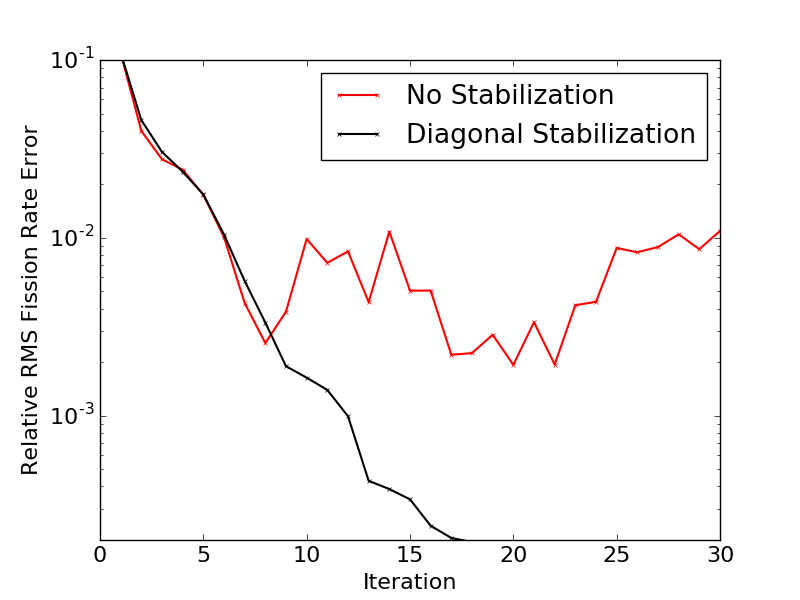
\includegraphics[width=0.65\linewidth]{figures/convergence/full-core-3D.png}
	\caption{Convergence behavior the full core \ac{BEAVRS} benchmark with and without Diagonal Stabilization ($\rho = 1/4$).}
	\label{fig:fc-3D}
\end{figure}

These results show that for the 3D full core \ac{PWR} problem, a stabilization technique is necessary in order to reach any reasonable convergence, especially when it is computationally infeasible to use a many-group \ac{CMFD} solver.

\section{Conclusion}

In this study, a theoretical analysis of source iteration convergence was presented which showed the possibility for source iteration instabilities. The theory was broadened to include source iterations without inner iterations. A new diagonal stabilization technique was presented which is substantially less conservative than previously proposed techniques. Realistic reactor physics problems were presented that showed instability with the source iteration process. The diagonal stabilization technique was shown to successfully stabilize the source iteration process without having much impact on convergence rate.

Results were also presented for convergence with \ac{CMFD} acceleration which showed that \ac{CMFD} acceleration without group collapse was able to stabilize the source iteration process. For \ac{CMFD} acceleration with a collapsed group structure, the previously discussed stabilization techniques were necessary to ensure convergence. In the case of full core \ac{PWR} problems, a collapsed group structure is attractive to reduce run time, necessitating a stabilization method to converge to a reasonable distribution.
